% Chương 3 — Huy. Nguồn: docs/research-design.md, data-contract.md, modeling-training-plan.md, ADR-001/008/014,
% SERVER_CONTEXT/*.md. Chỉ mô tả phương pháp; số liệu kết quả để ở Chương 4.
\chapter{Phương pháp thực hiện}\label{ch:method}

Chương này trình bày cách nhóm xây dựng và đánh giá mô hình nhận diện rủi ro bất mãn ẩn. Mục~\ref{sec:pipeline} phát biểu bài toán và mô tả quy trình tổng thể. Mục~\ref{sec:data} trình bày dữ liệu, cách xây dựng quần thể nghiên cứu và các biện pháp chống rò rỉ dữ liệu. Mục~\ref{sec:models} mô tả các mô hình, cách chia dữ liệu theo thời gian, hiệu chỉnh xác suất và chọn ngưỡng. Mục~\ref{sec:eval} trình bày các chỉ số đánh giá và giới hạn khi diễn giải kết quả.

% =====================================================================
\section{Quy trình triển khai và đặc tả hệ thống}\label{sec:pipeline}

\subsection{Phát biểu bài toán}

Nghiên cứu tập trung vào các đơn hàng Olist được giao đúng hoặc sớm hơn ngày dự kiến. Với nhóm đơn này, giao hàng trễ không còn là lời giải thích hiển nhiên cho một đánh giá thấp, nên sự không hài lòng nếu có là ``ẩn'' đối với bộ phận vận hành. Câu hỏi nghiên cứu chính là: \emph{chỉ dùng thông tin có sẵn tại thời điểm giao hàng, mô hình học máy có thể ước lượng rủi ro đơn hàng nhận đánh giá 1--2 sao tốt đến mức nào, và danh sách ưu tiên tạo ra từ mô hình có hiệu quả hơn các cách xếp hạng đơn giản hay không?}

Bài toán được định nghĩa hình thức như sau:
\begin{itemize}
  \item \textbf{Đơn vị học} là một sản phẩm trong đơn (item), định danh bởi \texttt{product\_item\_id} $=$ \texttt{order\_id} $+$ \texttt{order\_item\_id}.
  \item \textbf{Đơn vị chia dữ liệu và vận hành} là đơn hàng. Mọi item của cùng một đơn luôn nằm trong cùng một phân vùng dữ liệu.
  \item \textbf{Thời điểm dự đoán} $t_o$ là thời điểm đơn $o$ được giao cho khách (\texttt{order\_delivered\_\allowbreak customer\_date}).
  \item \textbf{Nhãn} $y_o = 1$ nếu đơn $o$ nhận đánh giá 1 hoặc 2 sao, $y_o = 0$ nếu nhận 3--5 sao. Ngưỡng này thống nhất với các nghiên cứu trước trên cùng bộ dữ liệu~\cite{orman2026}.
\end{itemize}

Olist chỉ ghi nhận đánh giá ở mức đơn hàng, không cho biết sản phẩm nào gây ra đánh giá thấp. Vì vậy mỗi item thừa hưởng nhãn của đơn chứa nó; đây là một \emph{nhãn yếu}. Điểm $\hat p_i$ của item $i$ được hiểu là rủi ro đơn nhận đánh giá thấp trong bối cảnh có item đó, không phải bằng chứng cho thấy item đó là nguyên nhân. Rủi ro của đơn được tổng hợp theo luật \texttt{max-v1}:
\begin{equation}\label{eq:maxv1}
  \hat{r}_o = \max_{i \in o} \hat{p}_i
\end{equation}
Luật lấy giá trị lớn nhất phản ánh giả định rằng chỉ cần một sản phẩm có vấn đề là đủ để khách đánh giá thấp cả đơn. Luật được đánh số phiên bản để có thể thay thế mà không làm thay đổi cách đánh giá.

Ngoài ra, việc khách có viết đánh giá hay không cũng là một quá trình tự chọn~\cite{li2008}: khách không đánh giá chưa chắc đã hài lòng. Do đó mô hình ước lượng rủi ro \emph{được quan sát} trong nhóm đơn có đánh giá, không ước lượng mức bất mãn tiềm ẩn của toàn bộ khách hàng.

\subsection{Quy trình tổng thể}

Hệ thống gồm hai luồng: luồng dữ liệu và học máy chạy theo lô, và luồng vận hành phục vụ nhân viên chăm sóc khách hàng (Hình~\ref{fig:arch}). Hai luồng chỉ gặp nhau tại cơ sở dữ liệu: luồng học máy ghi kết quả chấm điểm, luồng vận hành đọc kết quả đó.

Hình~\ref{fig:ml-flow} trình bày quy trình học máy theo bảy bước:
\begin{enumerate}
  \item \textbf{Nạp dữ liệu}: chín tệp CSV Olist được kiểm tra cấu trúc và nạp vào tầng bronze. Mỗi lần nạp có một manifest ghi lại mã băm tệp nguồn, nhờ đó cùng một tệp không bị nạp hai lần.
  \item \textbf{Biến đổi}: dbt chuẩn hóa dữ liệu ở tầng silver, tính đặc trưng ở tầng trung gian (intermediate) và tạo bảng \texttt{gold.ml\_modelling\_items} ở mức item.
  \item \textbf{Chia dữ liệu} theo thời gian dự đoán thành sáu phân vùng (mục~\ref{sec:models}).
  \item \textbf{Chọn mô hình} bằng kiểm định rolling-origin trong giai đoạn huấn luyện.
  \item \textbf{Hiệu chỉnh xác suất} và \textbf{chọn ngưỡng} trên các phân vùng riêng.
  \item \textbf{Chấm điểm}: mô hình tính điểm cho từng item, sau đó tổng hợp thành điểm đơn theo \texttt{max-v1}.
  \item \textbf{Ghi kết quả} vào bảng dự đoán trong PostgreSQL và đưa các đơn đủ điều kiện vào hàng đợi rủi ro.
\end{enumerate}

\begin{figure}[htbp]\centering
\begin{tikzpicture}[font=\footnotesize,
  box/.style={draw,rounded corners,fill=#1,minimum width=3.3cm,minimum height=0.85cm,align=center},
  box/.default=gray!10, node distance=0.45cm and 0.6cm, >={Latex}]
  \node[box=brown!20] (csv) {CSV Olist\\(9 bảng)};
  \node[box=brown!20,right=of csv] (bronze) {Bronze\\nạp + manifest};
  \node[box=gray!20,right=of bronze] (silver) {Silver\\chuẩn hóa};
  \node[box=yellow!30,below=of silver] (gold) {Intermediate $\rightarrow$ Gold\\\texttt{ml\_modelling\_items}};
  \node[box=blue!15,left=of gold] (split) {Chia theo thời gian\\6 phân vùng};
  \node[box=blue!15,left=of split] (cv) {Rolling-origin 3 fold\\chọn biến thể};
  \node[box=teal!20,below=of cv] (cal) {Hiệu chỉnh xác suất\\sigmoid / isotonic};
  \node[box=violet!20,right=of cal] (thr) {Chọn ngưỡng\\top 5\% / 20\%};
  \node[box=orange!25,right=of thr] (score) {Chấm điểm item\\$\rightarrow$ \texttt{max-v1}};
  \node[box=red!20,below=of thr] (db) {Bảng dự đoán\\$\rightarrow$ hàng đợi rủi ro};
  \draw[->] (csv) -- (bronze); \draw[->] (bronze) -- (silver); \draw[->] (silver) -- (gold);
  \draw[->] (gold) -- (split); \draw[->] (split) -- (cv); \draw[->] (cv) -- (cal);
  \draw[->] (cal) -- (thr); \draw[->] (thr) -- (score); \draw[->] (score) |- (db);
  \node[draw,dashed,fit=(csv)(gold),inner sep=4pt,label={[font=\scriptsize]above:Kho dữ liệu (PostgreSQL + dbt)}] {};
\end{tikzpicture}
\caption{Quy trình dữ liệu và học máy.}\label{fig:ml-flow}
\end{figure}

\begin{figure}[htbp]\centering
  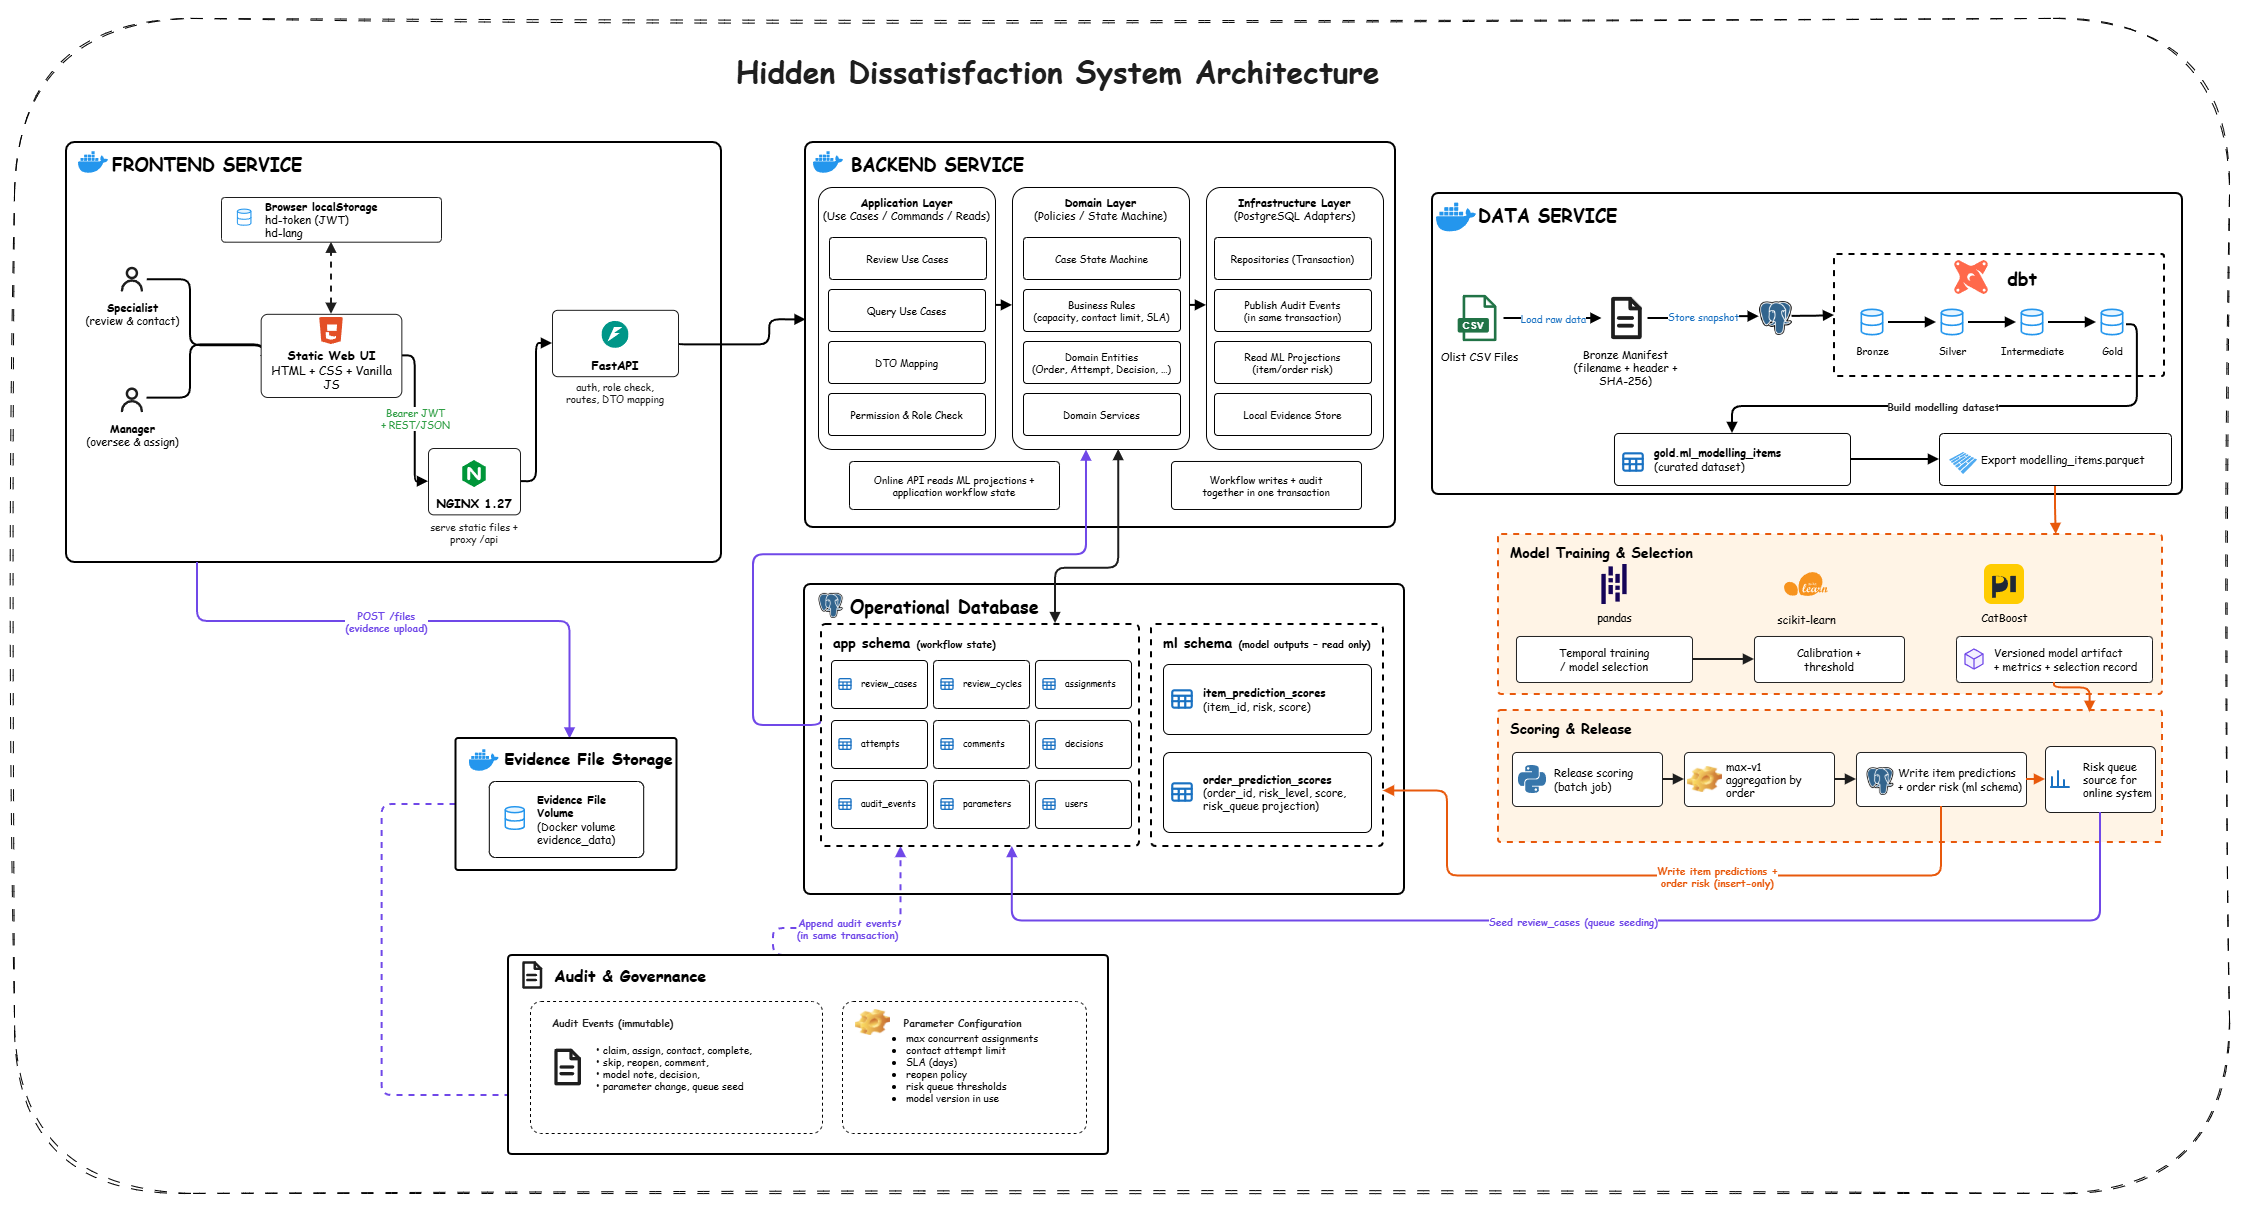
\includegraphics[width=\linewidth]{system-architecture}
  \caption{Kiến trúc tổng thể hệ thống}\label{fig:arch}
\end{figure}

\subsection{Đặc tả hệ thống}

Hệ thống được tổ chức theo kiến trúc phân lớp. Mỗi lớp chỉ đảm nhận một loại trách nhiệm, nhờ đó có thể thay mô hình học máy mà không phải sửa các lớp khác:
\begin{itemize}
  \item \textbf{Miền nghiệp vụ} (domain): điều kiện vào quần thể, ý nghĩa nhãn, các bất biến về thời gian. Lớp này không phụ thuộc thư viện dữ liệu hay mô hình.
  \item \textbf{Ứng dụng} (application): điều phối các ca sử dụng như nạp dữ liệu, huấn luyện, chấm điểm.
  \item \textbf{Hạ tầng} (infrastructure): đọc ghi PostgreSQL, tính đặc trưng, huấn luyện và lưu mô hình.
  \item \textbf{Giao diện} (interfaces): giao diện dòng lệnh (CLI) cho các tác vụ theo lô, và API cho ứng dụng web.
\end{itemize}

\textbf{Cơ chế chấm điểm theo lô.} Mô hình không được gọi theo thời gian thực. Một tác vụ theo lô chấm điểm toàn bộ item, tổng hợp điểm đơn bằng \texttt{max-v1}, gán mức \textsc{Cao}/\textsc{Trung bình}/\textsc{Thấp} theo ngưỡng đã chọn rồi ghi vào bảng dự đoán. Mỗi bản ghi lưu mã đơn, điểm rủi ro, mức ưu tiên và phiên bản mô hình, nên có thể truy vết kết quả về đúng lần huấn luyện. Cách làm này giữ ứng dụng web đơn giản và đảm bảo mọi người dùng nhìn thấy cùng một kết quả.

\textbf{Ứng dụng vận hành.} Backend viết bằng FastAPI, frontend bằng Angular, toàn bộ dịch vụ (PostgreSQL, API, frontend, tác vụ kho dữ liệu) được đóng gói bằng Docker Compose. Ứng dụng phục vụ hai vai trò: \emph{chuyên viên} (Specialist) nhận và xử lý đơn mức thấp và trung bình, \emph{quản lý} (Manager) giao đơn mức cao, điều chỉnh tham số vận hành và ra quyết định. Các chức năng chính gồm:
\begin{itemize}
  \item \textbf{Hàng đợi rủi ro}: danh sách đơn sắp xếp theo điểm rủi ro giảm dần, sau đó theo hạn SLA và thời gian chờ; có thể lọc theo mức rủi ro, trạng thái, người bán, danh mục.
  \item \textbf{Chi tiết đơn}: điểm của từng sản phẩm trong đơn, ghi nhận các lần liên lạc với khách và kết quả xử lý.
  \item \textbf{Dashboard và lịch sử kiểm toán}: tổng hợp tình trạng xử lý; mọi thao tác ghi đều sinh một sự kiện kiểm toán chỉ được thêm, không được sửa hay xóa.
\end{itemize}

Ba nguyên tắc được áp dụng xuyên suốt. Thứ nhất, backend kiểm tra mọi luật nghiệp vụ (quyền theo vai, giới hạn số đơn mỗi người, số lần liên lạc tối đa), kể cả khi frontend đã ẩn nút tương ứng. Thứ hai, không có API nào sửa được điểm rủi ro hay mức rủi ro do mô hình tạo ra. Thứ ba, các tham số vận hành như giới hạn số đơn và thời hạn SLA được lưu trong cơ sở dữ liệu và do quản lý điều chỉnh, không ghi cứng trong mã nguồn.

% =====================================================================
\section{Dữ liệu và công cụ}\label{sec:data}

\subsection{Nguồn dữ liệu}

Nghiên cứu sử dụng bộ dữ liệu công khai \emph{Brazilian E-Commerce Public Dataset by Olist}~\cite{olist2018}, gồm khoảng 99\,000 đơn hàng phát sinh trên các sàn thương mại điện tử tại Brazil từ năm 2016 đến 2018. Dữ liệu gồm chín bảng liên kết với nhau qua các khóa \texttt{order\_id}, \texttt{customer\_id}, \texttt{product\_id} và \texttt{seller\_id} (Bảng~\ref{tab:olist}). Bảng đơn hàng là trung tâm, ghi các mốc thời gian của vòng đời đơn: mua, duyệt, bàn giao cho đơn vị vận chuyển, giao cho khách và ngày giao dự kiến. Các mốc này là cơ sở để xác định thời điểm dự đoán và lọc đơn giao đúng hạn.

\begin{table}[htbp]\centering\small
\caption{Các bảng trong bộ dữ liệu Olist}\label{tab:olist}
\begin{tabular}{llr}
\toprule
Bảng & Độ chi tiết (một dòng là) & Số dòng \\
\midrule
\texttt{orders}         & một đơn hàng                          &    99\,441 \\
\texttt{order\_items}   & một sản phẩm trong đơn                &   112\,650 \\
\texttt{order\_payments}& một lần thanh toán của đơn            &   103\,886 \\
\texttt{order\_reviews} & một đánh giá                          &    99\,224 \\
\texttt{customers}      & một khách hàng theo đơn               &    99\,441 \\
\texttt{sellers}        & một người bán                         &     3\,095 \\
\texttt{products}       & một sản phẩm                          &    32\,951 \\
\texttt{geolocation}    & một tọa độ theo mã bưu chính          & 1\,000\,163 \\
\texttt{category\_translation} & một danh mục (tiếng Bồ Đào Nha -- Anh) & 71 \\
\bottomrule
\end{tabular}
\end{table}

Có hai đặc điểm cần lưu ý. Bảng đánh giá có 99\,224 dòng nhưng một số đơn có nhiều đánh giá và một số đơn không có đánh giá nào. Bảng thanh toán có thể có nhiều dòng cho một đơn khi khách trả bằng nhiều phương thức. Cả hai bảng vì vậy phải được gộp về mức đơn trước khi nối với bảng sản phẩm trong đơn.

\subsection{Xây dựng tập dữ liệu mô hình hóa}

Bảng mô hình hóa có độ chi tiết là item. Bảng thanh toán và bảng đánh giá vốn ở mức đơn, nên được gộp về một dòng mỗi đơn trước khi nối, tránh nhân bản item. Khi một đơn có nhiều đánh giá, nhóm chọn một đánh giá đại diện theo thứ tự ưu tiên: đánh giá đã được người bán trả lời, sau đó đánh giá có thời điểm trả lời hoặc tạo mới nhất, cuối cùng là mã đánh giá. Quy tắc này mang tính tất định, nên chạy lại luôn cho cùng kết quả.

Quần thể nghiên cứu gồm các đơn thỏa mãn đồng thời: (i) trạng thái \texttt{delivered}; (ii) ngày giao thực tế không muộn hơn ngày giao dự kiến; (iii) có đánh giá được tạo \emph{sau} thời điểm giao. Điều kiện (iii) loại các đánh giá tạo trước hoặc đúng lúc giao, vì khi đó không thể dự đoán trước khi nhãn xuất hiện. Bảng~\ref{tab:funnel} cho thấy số đơn và item còn lại sau mỗi bước lọc.

\begin{table}[htbp]\centering\small
\caption{Quá trình lọc quần thể nghiên cứu}\label{tab:funnel}
\begin{tabular}{lrr}
\toprule
Bước lọc & Đơn & Item \\
\midrule
Toàn bộ đơn hàng                          & 99\,441 & 112\,650 \\
Trạng thái \texttt{delivered}             & 96\,478 & 110\,197 \\
Giao đúng hoặc sớm hạn                    & 88\,644 & 101\,475 \\
Có đánh giá hợp lệ tạo sau thời điểm giao & 85\,420 &  97\,878 \\
\bottomrule
\end{tabular}
\end{table}

Tỉ lệ đơn nhận đánh giá thấp trong quần thể là 9,21\% (7\,865/85\,420), cho thấy bài toán mất cân bằng lớp rõ rệt. Bảng~\ref{tab:funnel} được dựng lại từ các tệp CSV gốc để kiểm toán. Snapshot dữ liệu đóng băng dùng cho huấn luyện có 85\,425 đơn và 97\,884 item, lệch 5 đơn và 6 item so với bản dựng lại. Nhật ký dbt xác nhận snapshot được tạo thành công và qua các kiểm tra về độ chi tiết và tính duy nhất, nhưng không lưu số đếm theo từng bước lọc nên chưa giải thích được chênh lệch này. Các thí nghiệm sử dụng số liệu của snapshot đóng băng.

\subsection{Đặc trưng và kiểm soát rò rỉ dữ liệu}

Mọi đặc trưng phải biết được tại thời điểm $t_o$. Nhóm cho phép các nhóm thông tin sau: thông tin đơn và thanh toán; thuộc tính sản phẩm, danh mục và người bán; vị trí của khách và người bán; giá, phí vận chuyển và cấu trúc đơn; thời gian giao và khoảng dư so với ngày dự kiến; và các đặc trưng lịch sử tính hoàn toàn từ sự kiện xảy ra trước $t_o$. Các đầu vào sau bị cấm: điểm, nội dung, tiêu đề và thời điểm của đánh giá; mọi hành động xảy ra sau đánh giá; các thống kê tính trên toàn bộ dữ liệu; và các mã định danh. Pipeline từ chối tự động mọi cột thuộc nhóm bị cấm hoặc không có trong danh sách khai báo. Hình~\ref{fig:leakage-timeline} minh họa ranh giới này.

\begin{figure}[htbp]\centering
\begin{tikzpicture}[x=1cm,y=1cm,font=\small,
  ev/.style={circle,fill,inner sep=1.5pt},
  lab/.style={align=center,font=\footnotesize}]
  \fill[green!12] (0,0) rectangle (9,1.2);
  \fill[red!12]   (9,0) rectangle (13.5,1.2);
  \node[lab,green!45!black] at (4.5,1.45) {Được dùng làm đặc trưng};
  \node[lab,red!60!black]   at (11.25,1.45) {Bị cấm (rò rỉ)};
  \draw[-{Latex}] (0,0) -- (13.7,0) node[right]{$t$};
  \node[ev] at (3,0) {};   \node[lab,below] at (3,-0.1) {Mua hàng};
  \node[ev] at (5.5,0) {}; \node[lab,below] at (5.5,-0.1) {Seller\\gửi hàng};
  \draw[very thick] (9,-0.3) -- (9,1.2);
  \node[lab,below] at (9,-0.3) {\textbf{Giao hàng}\\$t_o$ (thời điểm dự đoán)};
  \node[ev] at (11.5,0) {}; \node[lab,below] at (11.5,-0.1) {Tạo đánh giá\\(nhãn $y$)};
  \draw[|-|,thick,blue!60!black] (0.2,0.6) -- (9,0.6) node[midway,above,lab]{Lịch sử của seller/danh mục từ các đơn trước $t_o$};
\end{tikzpicture}
\caption{Ranh giới thời gian của đặc trưng. Đặc trưng lịch sử chỉ dùng sự kiện xảy ra trước $t_o$ (cận trên mở); thông tin đánh giá và mọi sự kiện sau $t_o$ bị loại.}
\label{fig:leakage-timeline}
\end{figure}

Đặc trưng lịch sử của người bán và danh mục (số đánh giá trước đó, điểm đánh giá trung bình, thời gian xử lý và giao hàng trung bình) chỉ được tính từ các đơn có cả thời điểm giao lẫn thời điểm đánh giá diễn ra \emph{trước} $t_o$ của đơn đang xét. Khi có ít hơn năm quan sát trước đó, giá trị trung bình được để trống và một cờ ``hỗ trợ thấp'' được bật, giúp mô hình phân biệt giữa ``không có lịch sử'' và ``lịch sử tốt''.

Tập đặc trưng cuối cùng (phiên bản \texttt{p5-item-v11-interactions}) gồm 61 đặc trưng chia thành bảy nhóm (Bảng~\ref{tab:features}). Việc đưa các đặc trưng về giao hàng và cấu trúc đơn được gợi ý từ các nghiên cứu cho thấy hiệu quả giao hàng ảnh hưởng đến điểm đánh giá~\cite{ravula2023,deshpande2023}, và giao hàng tách thành nhiều kiện có thể làm giảm sự hài lòng~\cite{brylla2022}. Olist không ghi thời điểm giao riêng cho từng item, nên số người bán và số sản phẩm trong đơn chỉ là đại diện gián tiếp cho việc tách đơn, không phải quan sát trực tiếp.

\begin{table}[htbp]\centering\small
\caption{Các nhóm đặc trưng trong tập cuối cùng}\label{tab:features}
\begin{tabular}{p{4.2cm}p{9cm}}
\toprule
Nhóm & Nội dung chính \\
\midrule
Cơ sở (24) & Giá, phí vận chuyển, thanh toán, thời gian giao, khoảng dư so với ngày dự kiến, kích thước sản phẩm, lịch sử đánh giá của seller và danh mục kèm cờ hỗ trợ thấp, danh mục, bang của khách \\
Tốc độ và độ biến động của seller (7) & Thời gian trung bình từ duyệt đơn đến bàn giao vận chuyển và đến khi giao, độ lệch chuẩn, hệ số biến thiên, tỉ lệ phí vận chuyển \\
Số lượng trong đơn (7) & Số seller, danh mục, sản phẩm; cờ nhiều item, nhiều seller, nhiều danh mục \\
Tỉ lệ trong đơn (4) & Tổng phí vận chuyển, tỉ trọng phí vận chuyển, tỉ trọng giá trị lớn nhất và nhỏ nhất của item \\
Mức độ tập trung (2) & Chỉ số Herfindahl--Hirschman theo danh mục và theo seller \\
Hình thái sản phẩm (13) & Thể tích, mật độ, tỉ lệ kích thước, phí vận chuyển trên giá và trên khối lượng, các cờ thiếu hoặc bằng không \\
Độ đầy đủ nội dung (4) & Độ dài tên và mô tả, số trường mô tả bị thiếu \\
\bottomrule
\end{tabular}
\end{table}
% Danh sách đầy đủ 61 cột: đưa vào Phụ lục (SERVER_CONTEXT/chapter3_evidence.md §5).

\subsection{Công cụ}

Pipeline được viết bằng Python 3.11 với pandas 2.3.3, NumPy 2.4.6 và PyArrow 21.0.0 để xử lý dữ liệu; scikit-learn 1.9.1 và CatBoost 1.2.10 để huấn luyện mô hình; joblib 1.6.0 để lưu mô hình. Kho dữ liệu dùng PostgreSQL với các phép biến đổi viết bằng dbt 1.8.10. Toàn bộ ranh giới thời gian, danh sách biến thể và siêu tham số được khai báo trong một tệp cấu hình TOML có quản lý phiên bản, thay vì nằm rải rác trong notebook. Mọi lần chạy dùng seed cố định 42 và giới hạn số luồng để kết quả lặp lại được. Mỗi lần chạy xuất một báo cáo JSON ghi lại cấu hình, số liệu theo phân vùng, chỉ số và mã commit Git. GPU chỉ được dùng cho các biến thể CatBoost; mô hình được giữ lại chạy trên CPU.

Kho dữ liệu được tổ chức theo kiến trúc medallion. Tầng \emph{bronze} lưu dữ liệu nguyên dạng từ các tệp CSV kèm manifest chống nạp trùng. Tầng \emph{silver} chuẩn hóa kiểu dữ liệu và gộp tọa độ theo mã bưu chính. Tầng \emph{intermediate} chứa các mô hình dbt tính quần thể nghiên cứu, đánh giá đại diện, đặc trưng lịch sử và các nhóm đặc trưng trong Bảng~\ref{tab:features}. Tầng \emph{gold} gồm các bảng sự kiện và chiều phục vụ dashboard (đơn hàng, sản phẩm trong đơn, thanh toán, đánh giá, người bán, sản phẩm, khách hàng) và bảng \texttt{ml\_modelling\_items} phục vụ huấn luyện. Sau mỗi lần build, dbt chạy các kiểm tra tự động về tính duy nhất của khóa và độ chi tiết của bảng; các đặc trưng lịch sử có kiểm thử đơn vị riêng để đảm bảo không dùng sự kiện từ tương lai.

% =====================================================================
\section{Mô hình và thuật toán}\label{sec:models}

\subsection{Mô hình cơ sở và ứng viên}

Nhóm so sánh các mô hình theo thứ tự độ phức tạp tăng dần:
\begin{itemize}
  \item \textbf{Mô hình theo tỉ lệ nền} (prevalence): dự đoán mọi item bằng tỉ lệ dương của tập huấn luyện. Mô hình này là mức sàn mà mọi ứng viên phải vượt qua.
  \item \textbf{Hồi quy logistic} với hai mức điều chuẩn $C \in \{0{,}1;\,1\}$.
  \item \textbf{Rừng ngẫu nhiên} (Random Forest) với hai cấu hình: (độ sâu 8, tối thiểu 5 mẫu mỗi lá) và (độ sâu 12, tối thiểu 10 mẫu mỗi lá).
  \item \textbf{HistGradientBoosting} với hai cấu hình: (L2 $=1$, 31 lá) và (L2 $=5$, 15 lá).
  \item \textbf{CatBoost} chạy trên GPU, dùng cơ chế xử lý biến phân loại có sẵn, với độ sâu 6, 8 và 10.
\end{itemize}

Bên cạnh mô hình, nhóm thử bốn chế độ huấn luyện: \emph{item-unweighted} (mỗi item có trọng số như nhau), \emph{order-weight} (trọng số mỗi item bằng nghịch đảo số item trong đơn, để mỗi đơn đóng góp như nhau), \emph{order-reference} và \emph{order-aggregate} (gộp item thành một dòng mỗi đơn trước khi huấn luyện). Chế độ order-aggregate được thêm vào vì nhãn và chỉ số chính đều ở mức đơn.

\subsection{Tiền xử lý}

Mỗi họ mô hình có một nhánh tiền xử lý riêng. Với hồi quy logistic và rừng ngẫu nhiên, biến số được điền giá trị thiếu bằng trung vị (hồi quy logistic có thêm chuẩn hóa), biến phân loại được điền bằng giá trị phổ biến nhất rồi mã hóa one-hot, bỏ qua các giá trị chưa gặp. Với HistGradientBoosting, biến phân loại được mã hóa thứ tự để giữ ma trận dày. CatBoost nhận trực tiếp biến phân loại. Mọi bước tiền xử lý được đặt trong cùng một pipeline với mô hình và chỉ được fit trên dữ liệu huấn luyện của từng fold, tránh để thống kê của tập kiểm định lọt vào quá trình huấn luyện.

\subsection{Xử lý mất cân bằng lớp}

Với tỉ lệ dương khoảng 9--14\%, nhóm xử lý mất cân bằng bằng trọng số lớp (ví dụ \texttt{class\_weight=balanced\_subsample} cho rừng ngẫu nhiên) kết hợp với chọn ngưỡng riêng, thay vì lấy mẫu lại dữ liệu. Lựa chọn này dựa trên hai bằng chứng. Thứ nhất, với các bộ phân loại mạnh như mô hình boosting, cân bằng dữ liệu bằng SMOTE hầu như không cải thiện so với việc tối ưu ngưỡng~\cite{elor2022smote}. Thứ hai, các phương pháp hiệu chỉnh mất cân bằng làm xác suất dự đoán bị lệch lên một cách có hệ thống, làm hỏng độ tin cậy của xác suất~\cite{vandengoorbergh2022}. Vì bài toán cần xác suất đáng tin để xếp hàng ưu tiên, SMOTE chỉ được xem là thí nghiệm phụ và chưa được đưa vào pipeline chính.

\subsection{Chia dữ liệu theo thời gian và lựa chọn mô hình}

Dữ liệu được sắp theo thời điểm dự đoán $t_o$ và chia thành sáu phân vùng liên tiếp (Bảng~\ref{tab:split}). Mỗi phân vùng là khoảng nửa mở $[\text{đầu}, \text{cuối})$ và mọi item của một đơn luôn nằm cùng phân vùng. Mỗi phân vùng chỉ phục vụ đúng một mục đích, nên không có quyết định nào được đưa ra trên dữ liệu đã dùng cho quyết định trước đó. Cách chia này khác với việc chia ngẫu nhiên 80:20 thường gặp trong các nghiên cứu trước trên Olist~\cite{orman2026}: chia ngẫu nhiên cho phép mô hình ``nhìn thấy tương lai'', nên thường cho kết quả lạc quan hơn thực tế triển khai.

\begin{table}[htbp]\centering\small
\caption{Phân vùng dữ liệu theo thời gian dự đoán}\label{tab:split}
\begin{tabular}{lllrrr}
\toprule
Phân vùng & Từ & Đến (không gồm) & Đơn & Item & Tỉ lệ dương \\
\midrule
Huấn luyện            & 2016-10-11 & 2017-10-01 & 23\,545 & 26\,708 & 10,13\% \\
Lựa chọn mô hình      & 2017-10-01 & 2017-12-01 &  8\,586 &  9\,957 & 11,92\% \\
Fit hiệu chỉnh        & 2017-12-01 & 2018-02-01 & 11\,759 & 13\,444 & 12,74\% \\
So sánh hiệu chỉnh    & 2018-02-01 & 2018-04-01 & 10\,623 & 12\,265 & 13,80\% \\
Chọn ngưỡng           & 2018-04-01 & 2018-06-01 & 12\,351 & 14\,319 & 11,61\% \\
Test niêm phong       & 2018-06-01 & 2018-09-01 & 18\,561 & 21\,191 & ẩn \\
\bottomrule
\end{tabular}
\end{table}

Trong giai đoạn huấn luyện, các biến thể được so sánh bằng kiểm định rolling-origin với cửa sổ mở rộng gồm ba fold (Hình~\ref{fig:temporal-folds}). Ở mỗi fold, mô hình học trên toàn bộ dữ liệu trước mốc cắt và được đánh giá trên đoạn ngay sau đó, mô phỏng đúng cách mô hình được dùng trong thực tế. Biến thể được chọn theo thứ tự ưu tiên: PR-AUC mức đơn (theo \texttt{max-v1}) trung bình qua các fold cao nhất; nếu ngang nhau thì chọn biến thể có Brier score thấp hơn; nếu vẫn ngang nhau thì chọn mô hình đơn giản hơn. Hiệu chỉnh xác suất và chọn ngưỡng không tham gia vào bước này.

\begin{figure}[htbp]\centering
\begin{tikzpicture}[x=0.62cm,y=1cm,font=\footnotesize]
  % trục: tháng 0 = 2016-10; 23 = 2018-09
  \def\seg#1#2#3#4{\fill[#3] (#1,0) rectangle (#2,0.6); \node[font=\scriptsize] at ({(#1+#2)/2},0.3) {#4};}
  \seg{0}{12}{blue!30}{Huấn luyện}
  \seg{12}{14}{orange!55}{A}
  \seg{14}{16}{teal!40}{B}
  \seg{16}{18}{teal!25}{C}
  \seg{18}{20}{violet!30}{D}
  \seg{20}{23}{red!50}{Test}
  % 3 fold rolling-origin trong train; mốc thật, đơn vị tháng từ 2016-10-01:
  % 2017-06-01=8.0, 2017-07-18=9.57, 2017-08-24=10.77, 2017-10-01=12.0
  \foreach \k/\s/\e in {1/8.0/9.57,2/9.57/10.77,3/10.77/12.0} {
    \fill[blue!30] (0,-0.4*\k) rectangle (\s,-0.4*\k+0.28);
    \fill[orange!55] (\s,-0.4*\k) rectangle (\e,-0.4*\k+0.28);
    \node[left] at (0,-0.4*\k+0.14) {Fold \k};
  }
  \draw[densely dotted] (8,-1.3) -- (8,-1.55) node[below,font=\scriptsize]{2017-06};
  \draw[-{Latex}] (0,-1.55) -- (23.6,-1.55);
  \foreach \m/\l in {0/2016-10,12/2017-10,14/2017-12,16/2018-02,18/2018-04,20/2018-06,23/2018-09}
    \draw (\m,-1.5) -- (\m,-1.6) node[below,rotate=40,anchor=north east,font=\scriptsize]{\l};
  \node[align=left,anchor=north west,font=\scriptsize] at (0,-2.7)
    {A: lựa chọn mô hình \quad B: fit hiệu chỉnh \quad C: so sánh hiệu chỉnh \quad D: chọn ngưỡng \quad Test: test niêm phong};
\end{tikzpicture}
\caption{Thiết kế chia dữ liệu theo thời gian. Ba fold rolling-origin với cửa sổ mở rộng nằm trong giai đoạn huấn luyện; đoạn kiểm định của các fold lần lượt bắt đầu ngày 2017-06-01, 2017-07-18 và 2017-08-24. Mọi sản phẩm của một đơn nằm cùng một phân vùng.}
\label{fig:temporal-folds}
\end{figure}

\subsection{Hiệu chỉnh xác suất và ngưỡng ưu tiên}

Trọng số lớp giúp mô hình chú ý đến lớp thiểu số nhưng làm xác suất đầu ra bị đẩy lên cao. Vì hàng đợi ưu tiên cần xác suất phản ánh đúng tỉ lệ thực tế, nhóm hiệu chỉnh xác suất sau khi đã chọn mô hình. Mô hình gốc được huấn luyện lại trên phân vùng huấn luyện và lựa chọn. Hai phương pháp hiệu chỉnh, sigmoid (Platt scaling) và isotonic, được fit trên phân vùng \emph{fit hiệu chỉnh}, rồi so sánh bằng Brier score trên phân vùng \emph{so sánh hiệu chỉnh} độc lập. Nếu không phương pháp nào cải thiện Brier score so với mô hình gốc, mô hình gốc được giữ nguyên. Tách riêng hai phân vùng giúp kết quả so sánh không bị lạc quan do đánh giá trên chính dữ liệu đã dùng để fit.

Ngưỡng ưu tiên được chọn trên phân vùng \emph{chọn ngưỡng}: các đơn thuộc 5\% điểm rủi ro cao nhất được gán mức \textsc{Cao}, các đơn còn lại trong 20\% cao nhất được gán mức \textsc{Trung bình}. Cách chọn theo tỉ lệ phần trăm gắn trực tiếp với năng lực xử lý của bộ phận chăm sóc khách hàng thay vì một ngưỡng xác suất cố định.

% =====================================================================
\section{Phương pháp đánh giá}\label{sec:eval}

Do lớp dương chỉ chiếm khoảng một phần mười, độ chính xác (accuracy) không có ý nghĩa: một mô hình dự đoán mọi đơn đều tốt đã đạt khoảng 90\%. Nhóm dùng ba chỉ số, tính trên đoạn kiểm định của từng fold rồi lấy trung bình qua ba fold.

\textbf{PR-AUC} (diện tích dưới đường cong precision--recall) là chỉ số chính, đo ở mức item và mức đơn (sau khi tổng hợp bằng \texttt{max-v1}). PR-AUC của một mô hình xếp hạng ngẫu nhiên xấp xỉ tỉ lệ dương, nên tỉ lệ dương của từng fold là mốc so sánh tự nhiên.

\textbf{Brier score} đo độ tin cậy của xác suất ở mức đơn:
\begin{equation}\label{eq:brier}
  \mathrm{BS} = \frac{1}{N}\sum_{j=1}^{N}\left(\hat{p}_j - y_j\right)^2
\end{equation}
trong đó $\hat p_j$ là xác suất dự đoán và $y_j \in \{0,1\}$ là nhãn thực tế; giá trị càng thấp càng tốt. Brier score cũng là tiêu chí so sánh các phương pháp hiệu chỉnh xác suất ở mục~\ref{sec:models}.

\textbf{Recall@5\%} đo hiệu quả ưu tiên: tỉ lệ đơn nhận đánh giá thấp nằm trong 5\% đơn có điểm rủi ro cao nhất. Mức 5\% tương ứng với nhóm ưu tiên \textsc{Cao}. Nếu chọn ngẫu nhiên 5\% số đơn, recall kỳ vọng chỉ là 5\%, nên đây là mốc để đánh giá giá trị của mô hình đối với bộ phận vận hành.

Các kết quả trình bày ở Chương~4 là kết quả trên các fold phát triển. Phân vùng test niêm phong chưa được dùng để đánh giá, vì vậy các con số mang tính thăm dò và chưa phải ước lượng cuối cùng về hiệu năng khi triển khai.
